\begin{frame}
	\frametitle{Molten Salt Fast Reactor}
		\textbf{Features}
		\begin{itemize}
			\item Fast-spectrum \gls{MSR} concept
			\item Can run on the open U/Pu, U/TRU or closed U/Th fuel cycles
			\item Primary fuel salt flows upwards through the central core
			region and separates into 16 smaller external loops towards the
			heat exchangers and pumps
			\item Radially surrounded by a tank of blanket salt consisting of
			fertile isotopes such as $^{232}$Th for breeding
		\end{itemize}
		\begin{columns}
			\column[t]{3.5cm}
			\begin{figure}
				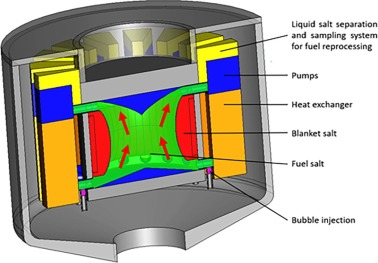
\includegraphics[width=\textwidth]{../paper/figures/MSFR}
				\caption{\gls{MSFR} concept}
			\end{figure}
			\column[t]{6.5cm}
			{\footnotesize
			\begin{table}[h]
				\caption{\footnotesize Specifications of the \gls{MSFR} design
				\cite{serp_molten_2014}.}
				\begin{tabular}{ l l }
				\hline
				Parameter & Value \\
				\hline
				Thermal/Electric output [MW$_{\text{th}}$/MW$_{\text{e}}$] &
				3000 / 1500 \\
				Salt volume [m$^3$] & 18 \\
				Salt fraction in core & 0.5 \\
				Number of circulation loops & 16 \\
				Nominal flow rate [kg s$^{-1}$] & 18500  \\
				Nominal circulation time [s] & 4.0 \\
				Inlet/outlet temperature [K] & 923 / 1023 \\
				Blanket volume [m$^3$] & 7.3\\
				\hline
				\end{tabular}
			\label{table:msfr}
			\end{table}
			}
		\end{columns}
\end{frame}